\section{Two sided matching markets}
\newcommand\tab[1][1cm]{\hspace*{#1}}

% introduce two sided matching

\begin{frame}
\frametitle{Two sided matching}
\centering
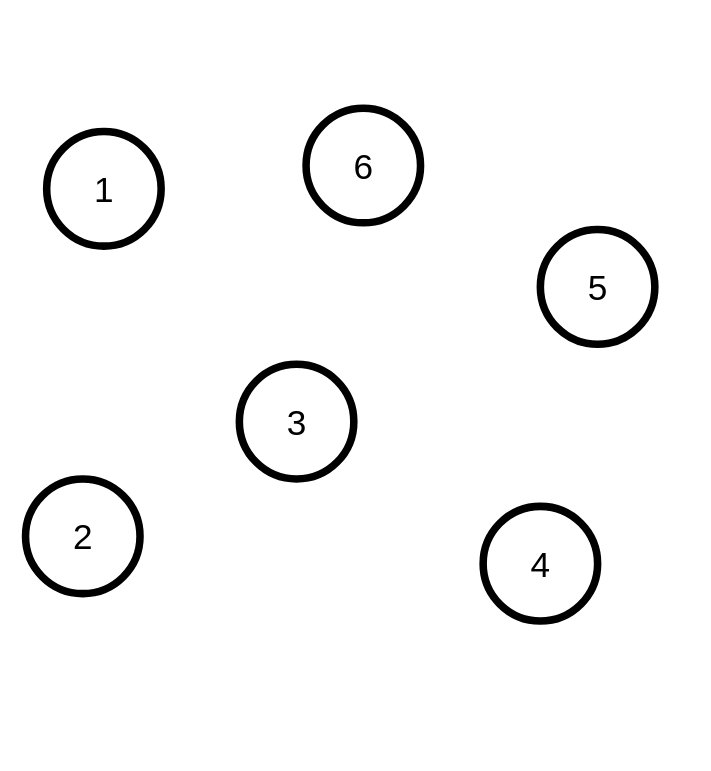
\includegraphics[width=5cm]{img/intro/agents.png}
\end{frame}

\begin{frame} 
\frametitle{Two sided matching}
\begin{itemize}
    \item Two disjoint sets of agents
\end{itemize}

\centering
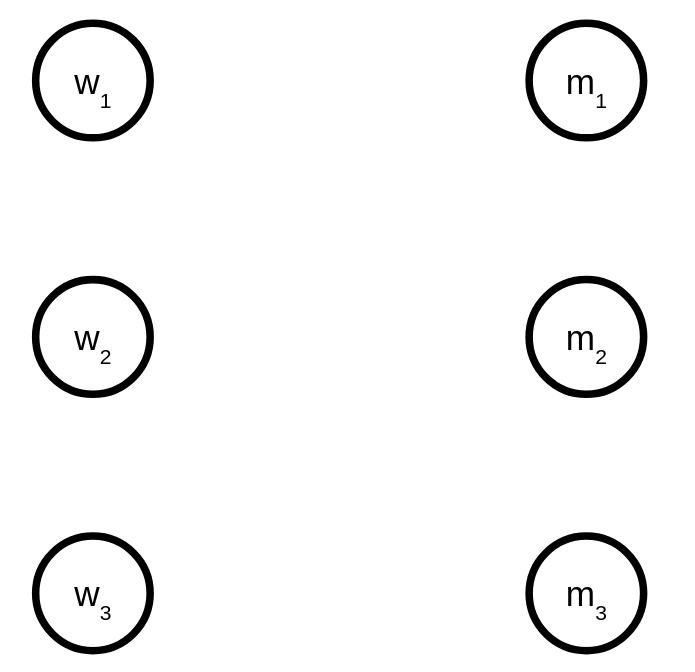
\includegraphics[width=5cm]{img/matching/twosided.png}
\end{frame}


\begin{frame} 
\frametitle{Two sided matching}
\begin{itemize}[<+->]
    \item Two disjoint sets of agents
    \item Strict preference orders  
    \item $w_1: m_2 \succ_{w_1} m_1 \succ_{w_1} m_3$ \tab $m_1: w_1 \succ_{m_1} w_3 \succ_{m_1} w_2$ \\
    $w_2: m_1 \succ_{w_2} m_2 \succ_{w_2} m_3$ \tab $m_2: w_3 \succ_{m_2} w_1 \succ_{m_2} w_2$ \\
    $w_3: m_1 \succ_{w_3} m_2 \succ_{w_3} m_3$ \tab $m_3: w_1 \succ_{m_3} w_3 \succ_{m_3} w_2$
    \item stable matching
\end{itemize}
\centering
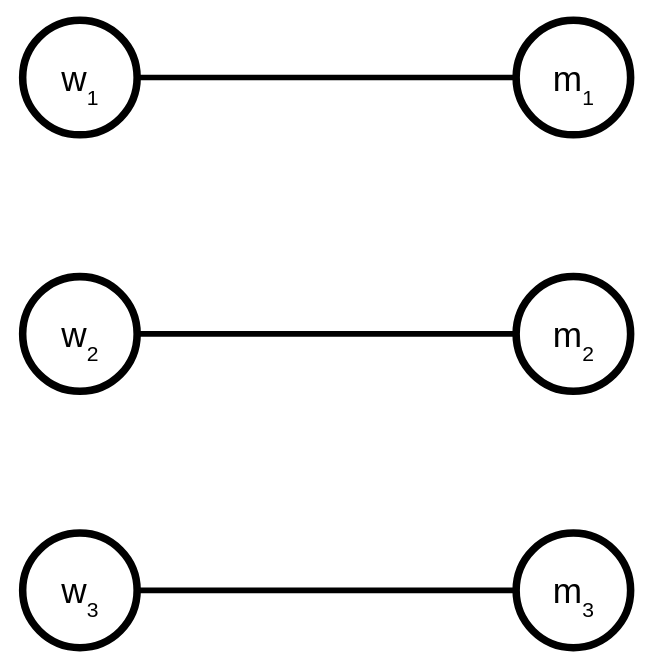
\includegraphics[width=5cm]{img/matching/unstable_matching.png}
\end{frame}

\begin{frame} 
\frametitle{Two sided matching}
\begin{itemize}
    \item Two disjoint sets of agents
    \item Strict preference orders 
    \item $w_1: m_2 \succ_{w_1} m_1 \succ_{w_1} m_3$ \tab $m_1: w_1 \succ_{m_1} w_3 \succ_{m_1} w_2$ \\
    $w_2: m_1 \succ_{w_2} m_2 \succ_{w_2} m_3$ \tab $m_2: w_3 \succ_{m_2} w_1 \succ_{m_2} w_2$ \\
    $w_3: m_1 \succ_{w_3} m_2 \succ_{w_3} m_3$ \tab $m_3: w_1 \succ_{m_3} w_3 \succ_{m_3} w_2$
    \item stable matching
\end{itemize}
\centering
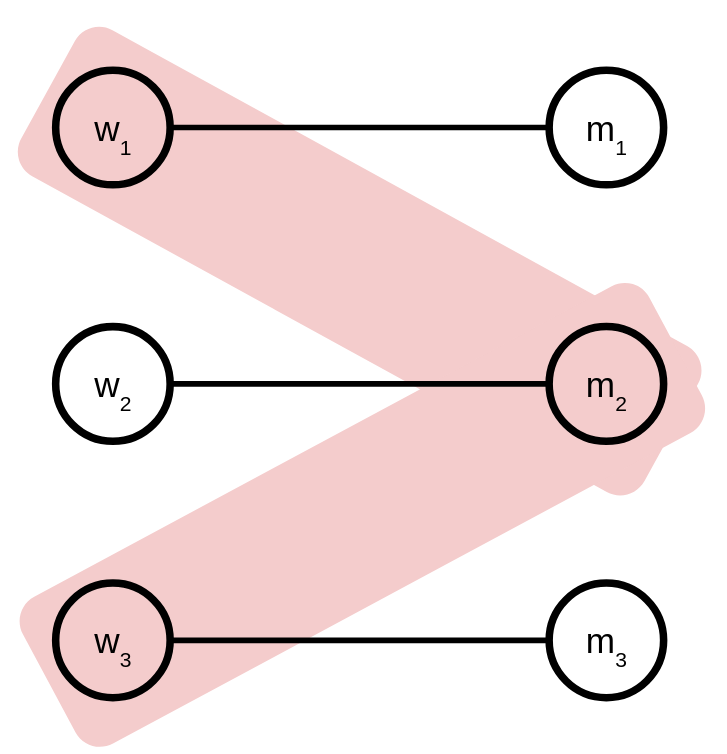
\includegraphics[width=5cm]{img/matching/blockingpairs.png}
\end{frame}


% deferred acceptance procedure
\begin{frame} 
\frametitle{Deferred Acceptance Procedure (DA)}
\centering
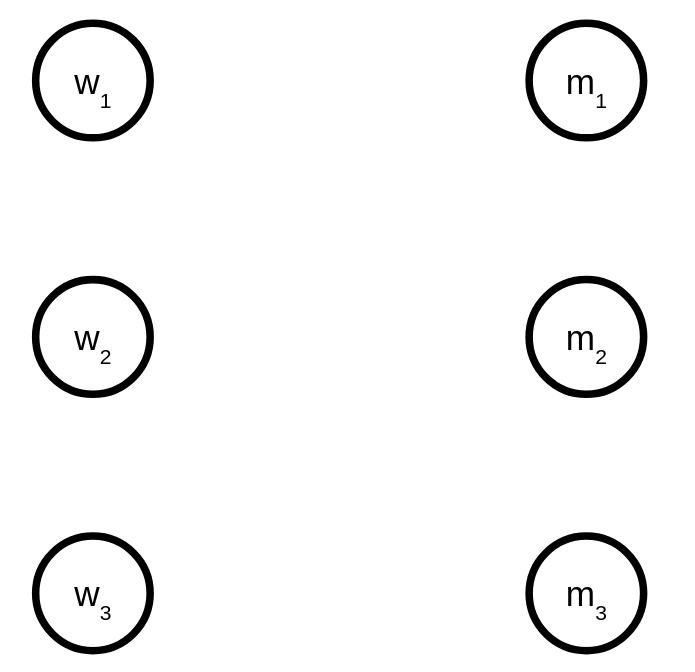
\includegraphics[width=6cm]{img/matching/twosided.png}
\end{frame}

% 1 step 
\begin{frame} 
\frametitle{Deferred Acceptance Procedure (DA)}
\centering
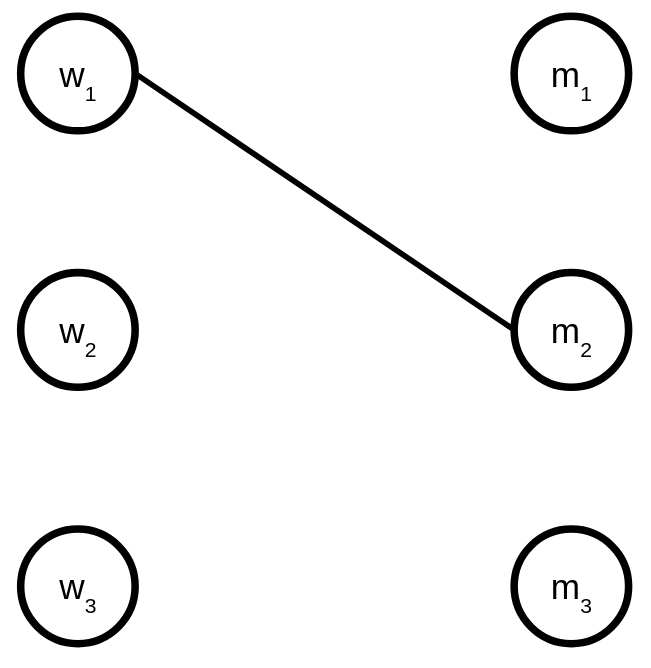
\includegraphics[width=6cm]{img/matching/da1.png}
\end{frame}

% 2 step 
\begin{frame} 
\frametitle{Deferred Acceptance Procedure (DA)}
\centering
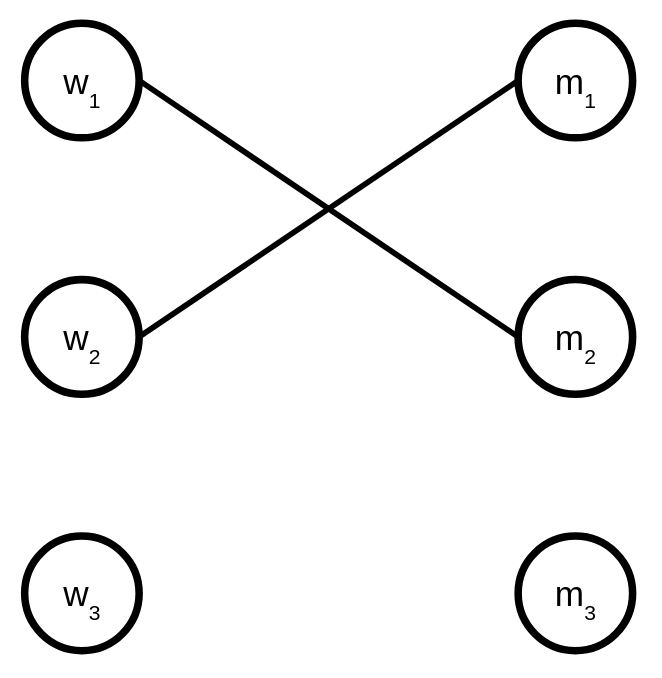
\includegraphics[width=6cm]{img/matching/da2.png}
\end{frame}

% 3 step 
\begin{frame} 
\frametitle{Deferred Acceptance Procedure (DA)}
\centering
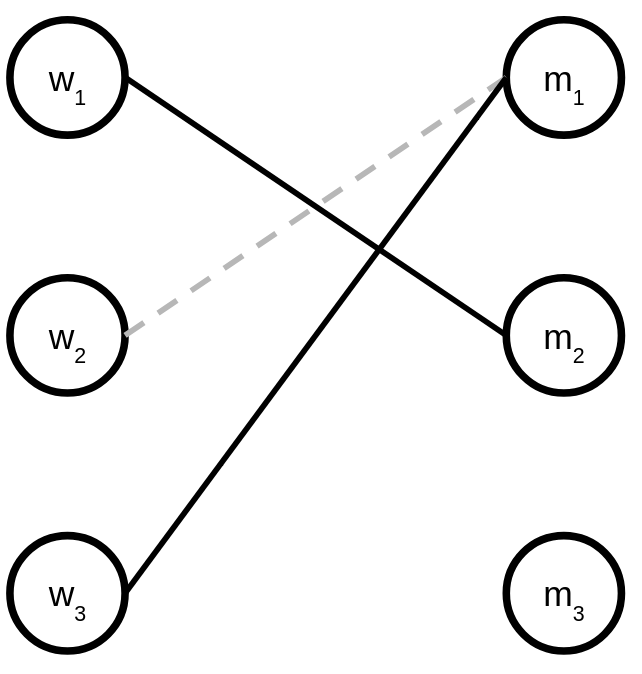
\includegraphics[width=6cm]{img/matching/da3.png}
\end{frame}

% 4 step 
\begin{frame} 
\frametitle{Deferred Acceptance Procedure (DA)}
\centering
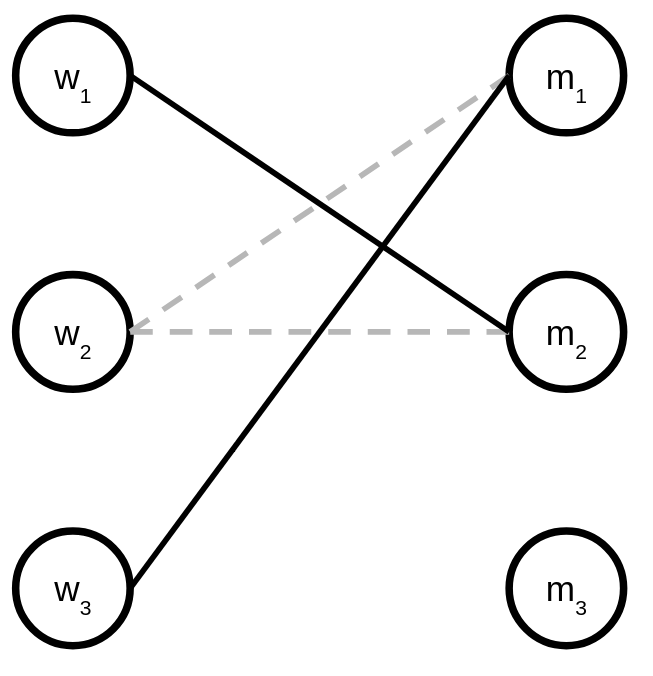
\includegraphics[width=6cm]{img/matching/da4.png}
\end{frame}

% 5 step 
\begin{frame} 
\frametitle{Deferred Acceptance Procedure (DA)}
\centering
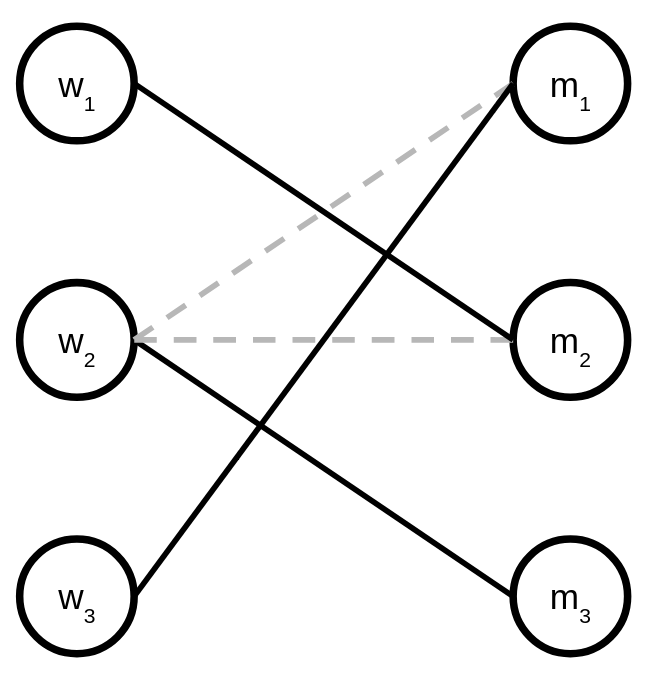
\includegraphics[width=6cm]{img/matching/da5.png}
\end{frame}

\begin{frame} 
\frametitle{Deferred Acceptance Procedure (DA)}
\begin{itemize}[<+->]
    \item Time complexity $O(nm), n:=|M|,m:=|W|$
    \item Matching is stable
    \item Matching is woman optimal
    \item not strategy proof!
    \item no matching is stable and strategy proof
\end{itemize}
\centering
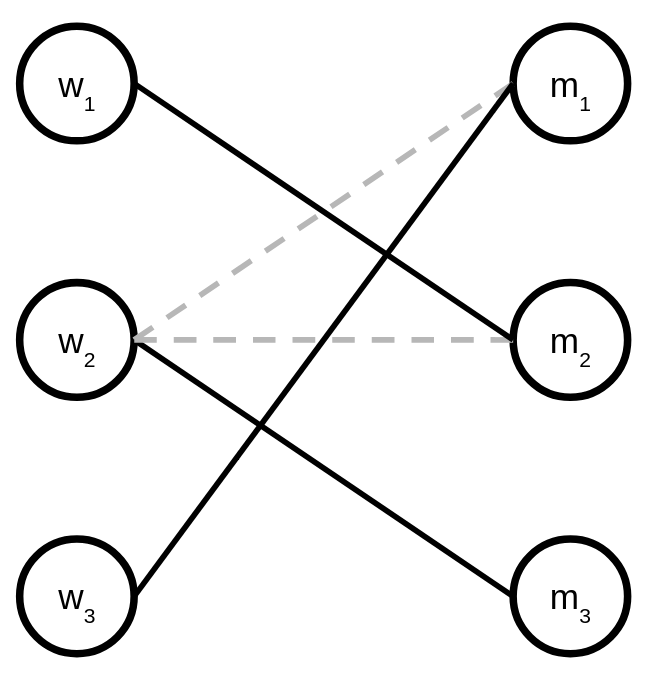
\includegraphics[width=5cm]{img/matching/da5.png}
\end{frame}

% prove that matching is stable 
\begin{frame}
\frametitle{Stability of matching \mu}
\begin{itemize}[<+->]
    \item Proof through contradiction, $\mu$ not stable
    \item Blocking pair $(w,m)$
    \item $m^* = \mu(w), w^* = \mu(m)$
    \item $m \succ_w m^*$
    \item $w$ proposes to $m$ before proposing to $m^*$ 
    \item $m$ must have rejected $w$ at some point
    \item $\implies \mu(m) = w^* \succ_m w$
    \item $(w,m)$ is not a blocking pair
\end{itemize}
\end{frame}

% perform counter example on flipchart (m1: w1,w2,w3) 
\begin{frame}
\frametitle{Incentives}
How can $m_1$ improve his match? \\
$w_1: m_2 \succ_{w_1} m_1 \succ_{w_1} m_3$ \tab $m_1: w_1 \succ_{m_1} w_3 \succ_{m_1} w_2$ \\
$w_2: m_1 \succ_{w_2} m_2 \succ_{w_2} m_3$ \tab $m_2: w_3 \succ_{m_2} w_1 \succ_{m_2} w_2$ \\
$w_3: m_1 \succ_{w_3} m_2 \succ_{w_3} m_3$ \tab $m_3: w_1 \succ_{m_3} w_3 \succ_{m_3} w_2$ \\
\centering
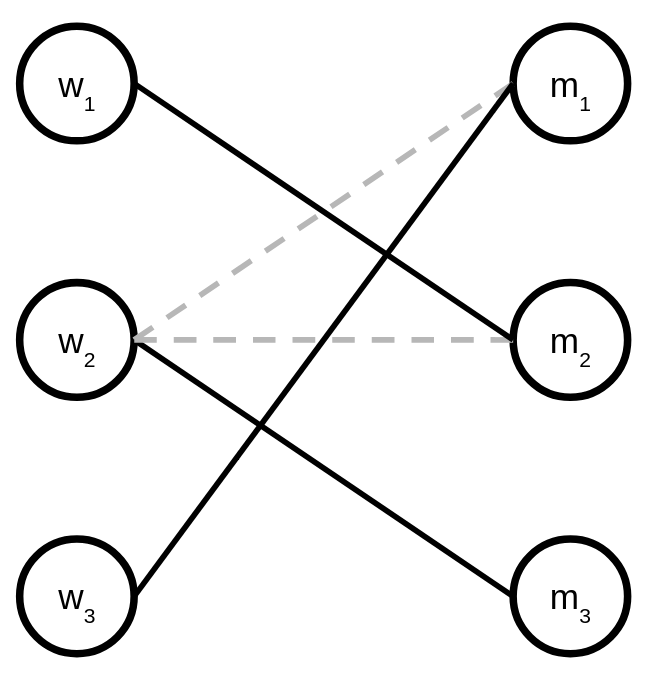
\includegraphics[width=6cm]{img/matching/da5.png}
\end{frame}

% write example of how m1 could improve
% 1
\begin{frame}{Incentives}
    $w_1: m_2 \succ_{w_1} m_1 \succ_{w_1} m_3$ \tab $m_1: w_1 \ \hat{\succ}_{m_1} \ w_2 \ \hat{\succ}_{m_1} \ w_3$ \\
    $w_2: m_1 \succ_{w_2} m_2 \succ_{w_2} m_3$ \tab $m_2: w_3 \succ_{m_2} w_1 \succ_{m_2} w_2$ \\
    $w_3: m_1 \succ_{w_3} m_2 \succ_{w_3} m_3$ \tab $m_3: w_1 \succ_{m_3} w_3 \succ_{m_3} w_2$ \\
    \centering
    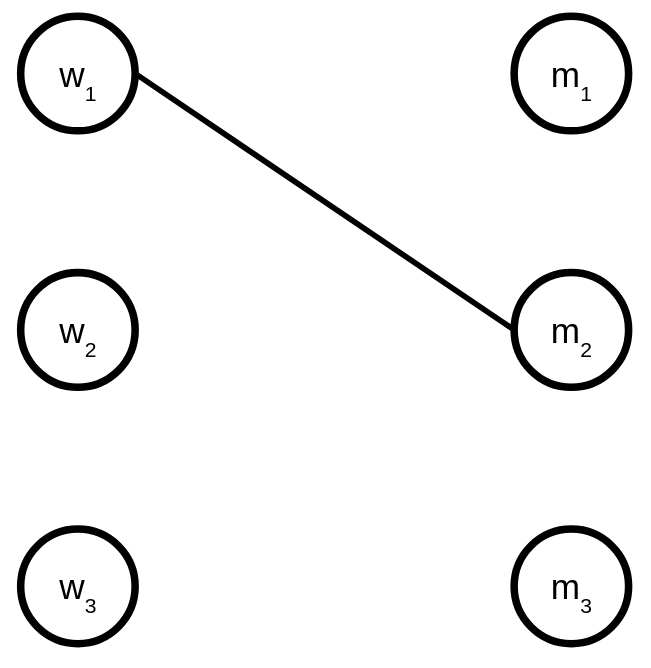
\includegraphics[width=6cm]{img/matching/da1.png}
\end{frame}

% 2
\begin{frame}{Incentives}
    $w_1: m_2 \succ_{w_1} m_1 \succ_{w_1} m_3$ \tab $m_1: w_1 \ \hat{\succ}_{m_1} \ w_2 \ \hat{\succ}_{m_1} \ w_3$ \\
    $w_2: m_1 \succ_{w_2} m_2 \succ_{w_2} m_3$ \tab $m_2: w_3 \succ_{m_2} w_1 \succ_{m_2} w_2$ \\
    $w_3: m_1 \succ_{w_3} m_2 \succ_{w_3} m_3$ \tab $m_3: w_1 \succ_{m_3} w_3 \succ_{m_3} w_2$ \\
    \centering
    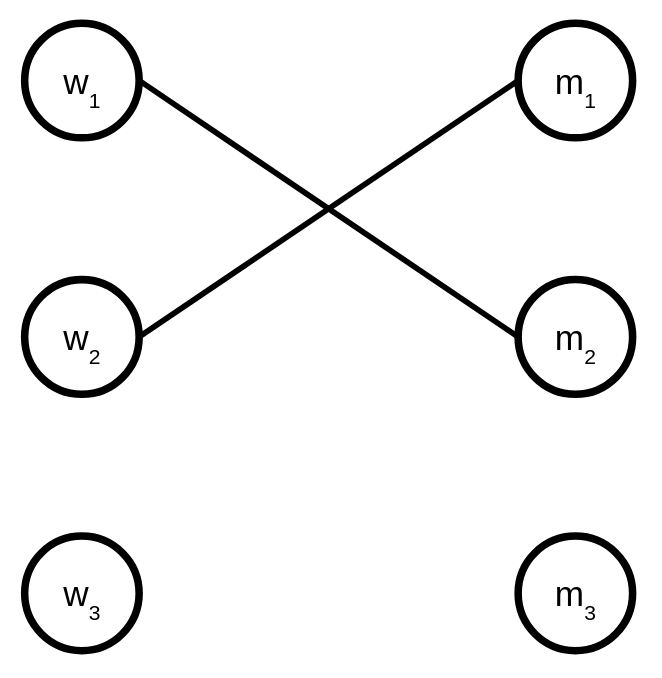
\includegraphics[width=6cm]{img/matching/da2.png}
\end{frame}

% 3
\begin{frame}{Incentives}
    $w_1: m_2 \succ_{w_1} m_1 \succ_{w_1} m_3$ \tab $m_1: w_1 \ \hat{\succ}_{m_1} \ w_2 \ \hat{\succ}_{m_1} \ w_3$ \\
    $w_2: m_1 \succ_{w_2} m_2 \succ_{w_2} m_3$ \tab $m_2: w_3 \succ_{m_2} w_1 \succ_{m_2} w_2$ \\
    $w_3: m_1 \succ_{w_3} m_2 \succ_{w_3} m_3$ \tab $m_3: w_1 \succ_{m_3} w_3 \succ_{m_3} w_2$ \\
    \centering
    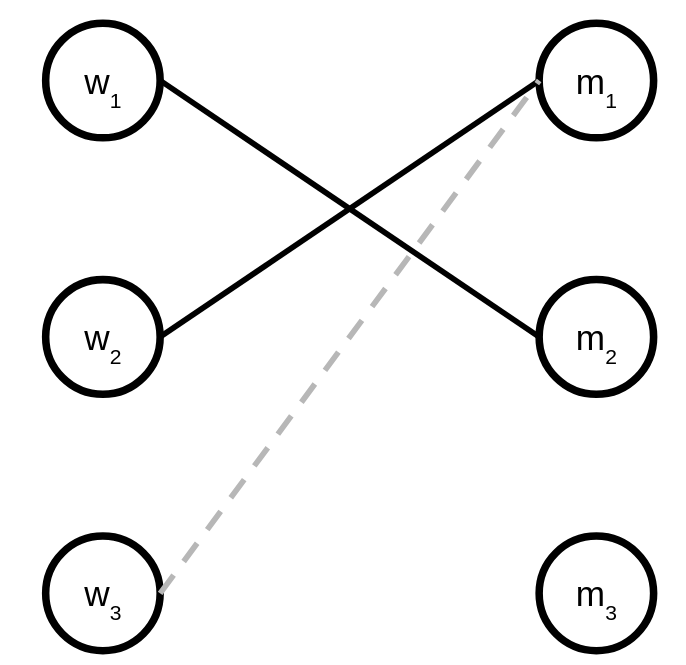
\includegraphics[width=6cm]{img/matching/dai3.png}
\end{frame}

% 4
\begin{frame}{Incentives}
    $w_1: m_2 \succ_{w_1} m_1 \succ_{w_1} m_3$ \tab $m_1: w_1 \ \hat{\succ}_{m_1} \ w_2 \ \hat{\succ}_{m_1} \ w_3$ \\
    $w_2: m_1 \succ_{w_2} m_2 \succ_{w_2} m_3$ \tab $m_2: w_3 \succ_{m_2} w_1 \succ_{m_2} w_2$ \\
    $w_3: m_1 \succ_{w_3} m_2 \succ_{w_3} m_3$ \tab $m_3: w_1 \succ_{m_3} w_3 \succ_{m_3} w_2$ \\
    \centering
    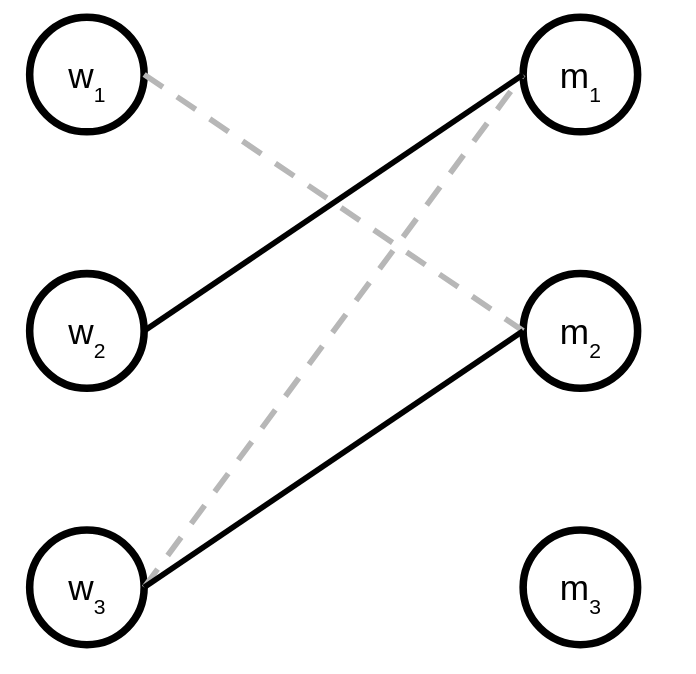
\includegraphics[width=6cm]{img/matching/dai4.png}
\end{frame}

% 5
\begin{frame}{Incentives}
    $w_1: m_2 \succ_{w_1} m_1 \succ_{w_1} m_3$ \tab $m_1: w_1 \ \hat{\succ}_{m_1} \ w_2 \ \hat{\succ}_{m_1} \ w_3$ \\
    $w_2: m_1 \succ_{w_2} m_2 \succ_{w_2} m_3$ \tab $m_2: w_3 \succ_{m_2} w_1 \succ_{m_2} w_2$ \\
    $w_3: m_1 \succ_{w_3} m_2 \succ_{w_3} m_3$ \tab $m_3: w_1 \succ_{m_3} w_3 \succ_{m_3} w_2$ \\
    \centering
    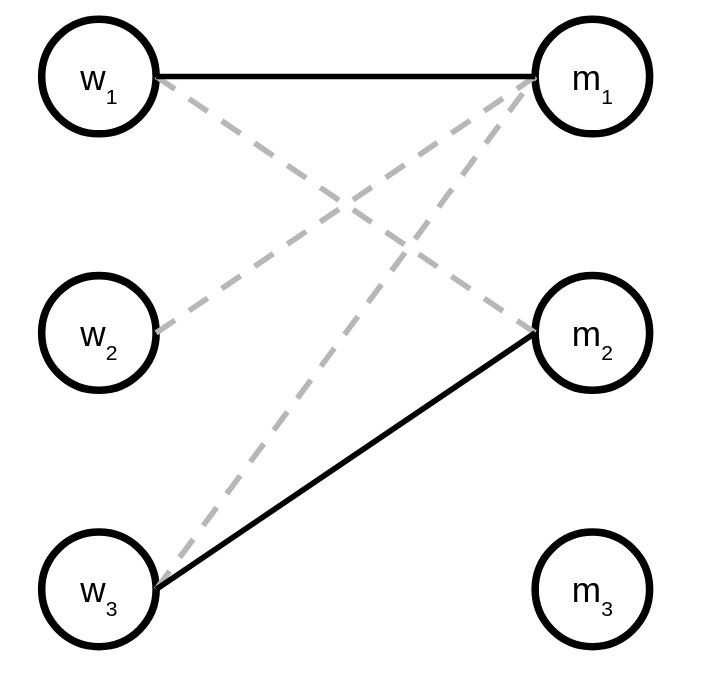
\includegraphics[width=6cm]{img/matching/dai5.png}
\end{frame}

% 6
\begin{frame}{Incentives}
    $w_1: m_2 \succ_{w_1} m_1 \succ_{w_1} m_3$ \tab $m_1: w_1 \ \hat{\succ}_{m_1} \ w_2 \ \hat{\succ}_{m_1} \ w_3$ \\
    $w_2: m_1 \succ_{w_2} m_2 \succ_{w_2} m_3$ \tab $m_2: w_3 \succ_{m_2} w_1 \succ_{m_2} w_2$ \\
    $w_3: m_1 \succ_{w_3} m_2 \succ_{w_3} m_3$ \tab $m_3: w_1 \succ_{m_3} w_3 \succ_{m_3} w_2$ \\
    \centering
    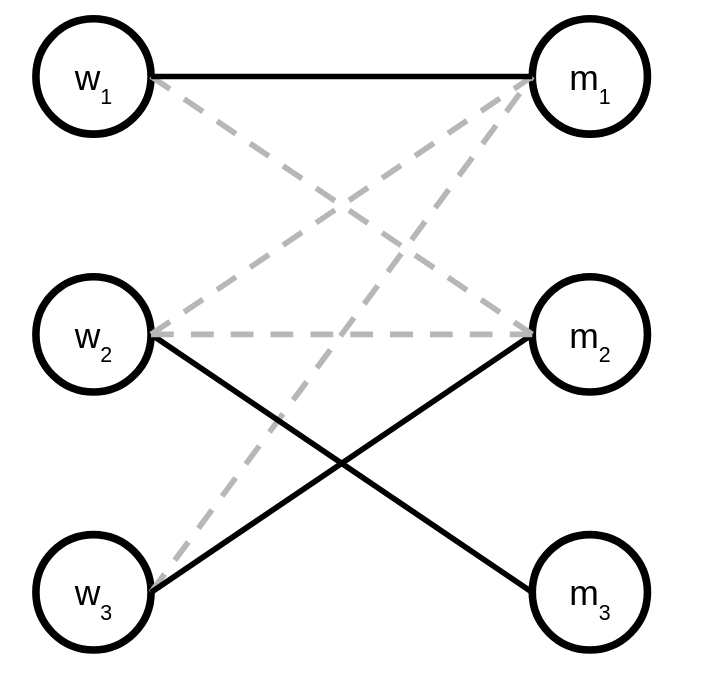
\includegraphics[width=6cm]{img/matching/dai6.png} \\
    Before: $(w_3,m_1)$, \\ after: $(w_1,m_1)$
\end{frame}